\chapter{Casi d'uso}

\section{UC1}

\section{UC2 - Selezione tipo di grafico}
\begin{figure}[H]
 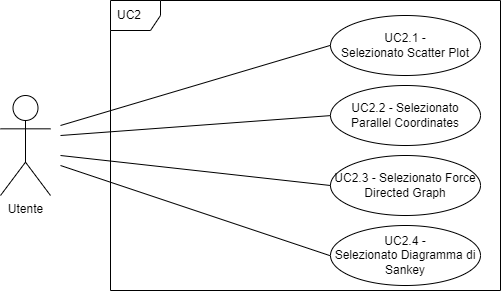
\includegraphics[width=\textwidth]{uc2.png}
 \vspace{-5mm}
 \caption*{Figura 2: UC2 - Selezione tipo di grafico}
\end{figure}
 \begin{itemize}
     \item \textbf{Descrizione:} Viene visualizzata la scelta della tipologia di grafico;
     \item \textbf{Attore primario:} Utente;
     \item \textbf{Precondizioni:} Il sistema è stato inizializzato [UC1].
     \item \textbf{Postcondizioni:} Viene selezionato il grafico desiderato e l'utente può procedere con la scelta delle dimensioni del grafico [UC3];
     \item \textbf{Scenario principale:} L'utente sceglie la visualizzazione più consona tra quelle disponibili;
     \item \textbf{Generalizzazioni:} L'utente può selezionare una delle seguenti opzioni:
     \begin{enumerate}
         \item \textit{Scatter Plot};
         \item \textit{Parallel Coordinates};
         \item \textit{Force Directed Graph};
         \item \textit{Diagramma di Sankey}.
     \end{enumerate}
 \end{itemize}
 
\section{UC3}

\section{UC4}

\section{UC5}

\section{UC6}

\section{UC7}
